\documentclass[11pt]{article}
\usepackage[table]{xcolor}  % load xcolor before anything else
\usepackage[most]{tcolorbox}
\usepackage{setspace}  %line spacing
\usepackage{titling}
\usepackage{graphicx}
% \usepackage{parskip}    %spaced paragraphs
\usepackage{csquotes}   %babel wanted it
\usepackage{emptypage} % prevent page numbers and headings on empty pages
\usepackage{float}
\usepackage{censor}
\usepackage{amsmath}
\usepackage{fontawesome}
\usepackage{pdfpages} % insert pdf 
\usepackage[titletoc]{appendix}

\usepackage[hang,flushmargin]{footmisc}     % footnote editing

\usepackage[font=small,labelfont=bf]{caption} % caption size 
\usepackage{subcaption}
\setlength{\belowcaptionskip}{-5pt}

\usepackage[hidelinks]{hyperref}  %have a review of this
\hypersetup{%
%   citecolor=black,
  colorlinks=false,
%   linkcolor=black,
%   urlcolor=black
}
\usepackage[nameinlink]{cleveref}

\usepackage{geometry}
\geometry{a4paper, margin=2.5cm}

\usepackage{fontspec}
\setmainfont[ 
    Mapping=tex-text,
    BoldFont={HelveticaNowText-Regular},
    ItalicFont={HelveticaNowText-LightItalic},
    BoldItalicFont={HelveticaNowText-RegIta}
]{[HelveticaNowText-Light]}

\usepackage{fancyhdr}   %footer
\fancypagestyle{myheadings}{%
    \fancyhf{}
    \renewcommand{\headrulewidth}{0.5pt}
    \renewcommand{\footrulewidth}{0pt}
    \addtolength{\headheight}{2pt}
    \fancyhead[L]{\leftmark}
    \fancyhead[R]{1922268}
    \cfoot{\thepage}
}
\pagestyle{myheadings}

\usepackage{enumitem}   %reduce list spacing
\setlist{nosep} 

\usepackage[
    backend=biber,
    % style=numeric-comp,
    % style = vancouver,
    style = science,
    % style=draft,
    % style = authoryear-icomp,
    maxnames=2, minnames=2,
    % doi=false,
    sorting=none
]{biblatex}   %bibliography
\usepackage{xurl} % break urls. load after biblatex
\addbibresource{../Report/extras/refs.bib}

\usepackage[
    separate-uncertainty=true,
    multi-part-units=single
    ]{siunitx}
\sisetup{
    detect-all,
    per-mode=symbol-or-fraction,
    tight-spacing,
    quantity-product =
    % number-unit-product=\,
    % space-before-unit=false
}
\DeclareSIUnit{\mAh}{mAh}

\usepackage{xltabular}
\usepackage{multirow}
\newcolumntype{Y}{>{\centering\arraybackslash}X}
\newcolumntype{Z}{>{\raggedright\arraybackslash}X}

\definecolor{titlepagecolour}{HTML}{003D99}
\definecolor{tableh1}{HTML}{dae3eb} %table grey
\definecolor{tableh2}{HTML}{b3ccf5} %table bluegrey
\definecolor{titleblue}{HTML}{1b1787} % blue
\definecolor{tableg}{HTML}{309c3d} % green
\definecolor{tablea}{HTML}{ed901f} % amber
\definecolor{tabler}{HTML}{f2422e} % red

\usepackage[british]{babel} 

\usepackage{pgfgantt}
\setganttlinklabel{s-s}{}
\setganttlinklabel{f-s}{}
\setganttlinklabel{f-f}{}

\usepackage{titlesec} 
\titlespacing\section{0pt}{12pt plus 4pt minus 2pt}{0pt plus 2pt minus 2pt}
\titlespacing\subsection{0pt}{12pt plus 4pt minus 2pt}{0pt plus 2pt minus 2pt}
\titlespacing\subsubsection{0pt}{12pt plus 4pt minus 2pt}{0pt plus 2pt minus 2pt}
\titlespacing\paragraph{0pt}{10pt plus 4pt minus 2pt}{10pt plus 2pt minus 2pt}

\begin{document}
\onehalfspacing

\section{Aims and objectives}

In this section, the aim and objectives set out in the thesis will be compared 
to the material achievements of the project. As these were both set out in list format,
they will be assessed on a per-point basis. 
Success of a give point is
determined by whether it was met \fcolorbox{black}{tableg}{\rule{0pt}{5pt}\rule{5pt}{0pt}}\,, 
unmet \fcolorbox{black}{tabler}{\rule{0pt}{5pt}\rule{5pt}{0pt}}\,, 
or somewhat met \fcolorbox{black}{tablea}{\rule{0pt}{5pt}\rule{5pt}{0pt}}\,. 

{\small
\begin{xltabular}{\linewidth}{|>{\raggedright\arraybackslash}p{4cm}|>{\color{white}}Z|}
    
    \hline
    \rowcolor{tableh2}
    Aim & \textcolor{black}{Remarks} \\
    \hline
    \endhead
    \endfoot

    \rowcolor{tableh1}
    \multicolumn{2}{|c|}{Fundamentals - minimum requirements to demonstrate the viability of the product.} \\
    \hline
    Obtain GPS location. & \cellcolor{tableg}The tracker obtains accurate GPS coordinates, within \qty{5}{\m}, 
        and is capable of including information like altitude, speed, and whether the reported location is `current'. \\ \hline
    Transmit location to a receiver via LoRa. & \cellcolor{tableg}Information is successfully transmitted via LoRa,
        however there is a small issue with occasional corruption of packets. \\ \hline    
    Continue transmission remotely for a significant period of time. & \cellcolor{tableg}Battery life allows transmission of up to 15 hours. \\ \hline    
    Transmit at a regular interval. & \cellcolor{tableg}The last updated location is  transmitted every \qty{5}{\s}. \\ \hline    

    \rowcolor{tableh1}
    \multicolumn{2}{|c|}{\parbox{12cm}{\centering Improvements - upgrades to the product to improve the user's quality of life when using the product.}} \\
    \hline
    Ergonomics for owner and pet (fitting and wearing). & \cellcolor{tabler}While a case was designed and houses the components 
        quite well, the primary aim was protection of the electronics during testing, as opposed to suitability for this use. \\ \hline
    Stability of the system (high uptime). & \cellcolor{tablea}The system is capable of running unattended for long periods of 
        time, however only the receiving end has any error handling capabilities. While it is unlikely for the transmitter 
        to crash for any reason, this has not been stress tested in any manner. \\ \hline
    Installable by an average person. & \cellcolor{tablea}Setting up the antenna or other system components is 
        not particularly difficult. The system overall could benefit from tooling (e.g. a base for the antenna) to 
        make this viable. Furthermore, accessing the receiver software to run it requires some knowledge of Bash, 
        which is not a fair expectation of the average person. \\ \hline
    Location information easily viewable. & \cellcolor{tablea}The location information is not difficult to see since it is
        stored plain-text in a file on the receiver. It also is not exactly easy, either, for the same reasons as above. \\ \hline
    
    \rowcolor{tableh1}
    \multicolumn{2}{|c|}{Production - requirements to ensure the product is suitable for manufacture.} \\
    \hline
    General safety and suitability to be worn. & \cellcolor{tabler}This follows ergonomics, wherein the case is not designed 
        to be worn at the stage that it is at as it cannot be attached in any way.
        It therefore has not been assessed for more than a superficial safety check (i.e. 
        the battery wires will not cross over and cause a fire). \\ \hline
    Resistance to damage and weather. & \cellcolor{tablea}It offers no protection from the environment. However, 
        the electronics are protected from damage and, by separation via insulating plastic, the user is protected from the electronics.  \\ \hline
    Certification requirements and law compliance. & \cellcolor{tabler}Not considered. \\ \hline
    Scale considerations, especially manufacturing. & \cellcolor{tabler}Not considered. \\ \hline     
    
    \caption{Aims evaluation}
    \label{table:aimeval}

\end{xltabular}
\vspace{-11pt}
}

{\small
\begin{xltabular}{\linewidth}{|>{\raggedright\arraybackslash}p{5cm}|>{\color{white}}Z|}
    \hline
    \rowcolor{tableh2}
    Objective & \textcolor{black}{Remarks} \\
    \hline
    \endhead
    \endfoot

    \hline
    Research cat characteristics, like roaming distances and time spent outdoors. & \cellcolor{tableg}This was well met,
        with the level of detail in research appropriate for defining the required specification points for the tracker. \\ \hline
    Research LoRa radio requirements for use, and competitive products. & \cellcolor{tableg}The exact details of the workings of LoRa 
        radio were not delved into deeply due to limited relevance, however an overview was provided. Research into alternative products and patents 
        was of sufficient depth to justify the relevance of the tracker. \\ \hline
    Design the system on a macroscopic level to inform hardware and software requirements. 
        This may include defining a specification of requirements the tracker must achieve. 
        & \cellcolor{tableg}A general overview was provided, including a software flowchart and hardware block diagram, so the 
        tracker can be understood in generality. A detailed specification was also written using the aims and research as a foundation. \\ \hline
    Develop the tracker such that it meets the outlined aims. & \cellcolor{tablea}Some of the specification points were met, but not all of them. 
        The aims' evaluation in \cref{table:aimeval} provides a general overview of this, as the specification is essentially a more granular version of the 
        aims. The tracker did meet some of the core aims, and with further work, could certainly meet outstanding points. The aims may have been 
        too ambitious in scope given the time available, however nothing impossible was specified. \\ \hline
    Perform tests to verify the efficacy of the tracker. & \cellcolor{tablea}Various tests were performed to ascertain different characteristics.
        This included testing the lifespan and distance-transmission capabilities. The distance tests were not sufficiently thorough 
        in order to draw solid conclusions about the tracker. This largely came down to time constraints (i.e. project development 
        ended at this objective). The tracker would certainly 
        have benefitted from a more thorough suite of tests on this characteristic. That is not to say the data gathered was entirely useless. 
        With confidence, the tracker works in very poor conditions within \qty{175}{\m}. \\ \hline
    Develop a PCB for the tracker to minimise form-factor, and produce adequate casing
        for it to be fitted to a pet collar or harness. This includes verifying basic functions
        again, in addition to suitability for intended use on an animal. & \cellcolor{tabler}As time ran out for test thoroughness in the previous 
        objective, from hereon no further points were tackled. The plan was to lift the components of the tracker onto a PCB that 
        would have minimised the size, and then develop casing around it that would be useable with a harness, however this could not be attempted 
        due to the time available. Therefore, this point in its entirety was not engaged with. \\ \hline
    Gain required certifications for the product to be moved to manufacture, and design
        a manufacturing plan. & \cellcolor{tabler}This objective would have defined the tracker to a point where it was potentially patentable,
        however was not addressed at all due to where development for the project had to end.  \\ \hline
    
    \caption{Objectives evaluation}\label{table:objeval}
\end{xltabular}
\vspace{-11pt}
}

Taking an overview of success, the project was generally meeting the set out aims and 
objectives, especially so with the earlier ones. Completion of each point began to suffer 
as the project progressed, leading to the more ambitious goals to not be attempted. 
Following this project on, these unmet points would prove an excellent extension, and 
there is nothing to suggest they would not be achievable if given enough time. 

\section{Project management}
Time constraints have been mentioned a number of times to this point. 
Project development was completed in a very short timespan, with development to produce 
the absolute minimum viable product completed over the space of a weekend. 
This may suggest rushed and therefore incomplete or buggy code, however this is not the case.
The majority of the working and useable code was completed to a reasonable standard extremely quickly, 
and only required minor improvements from thereon. 
This is also the case for much of the rest of development, with many major steps taken quickly and developed to a reasonable
level of polish. 

The issue largely came down to hardware delivery delays. While this was somewhat expected and accounted for,
the true extent was the entirety of Term 1 lost waiting for a hardware delivery. 
When the hardware did arrive, development progressed very quickly from thereon.
\begin{figure}[htbp!]
    \noindent\resizebox{\textwidth}{!}{
    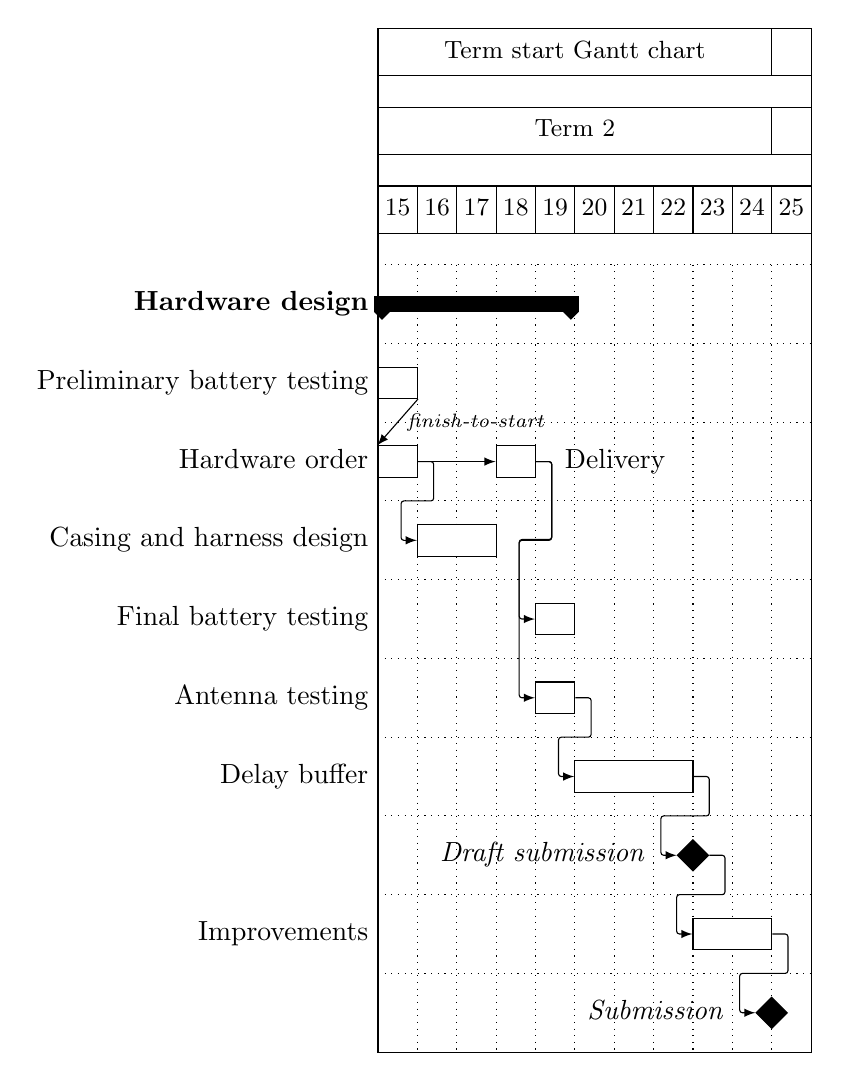
\begin{tikzpicture}[x=.5cm, y=.5cm]
        \begin{ganttchart}[
            hgrid, 
            vgrid,
            bar inline label node/.append style={right=5mm},
            milestone inline label node/.append style={left=5mm}
            ]{1}{11}
            \gantttitle{Term start Gantt chart}{10} \gantttitle{}{1}\\
            \gantttitle{Term 2}{10} \gantttitle{}{1}\\
            \gantttitlelist{15,...,25}{1} \\
        
            \ganttgroup{Hardware design}{1}{5} \\
            \ganttbar{Preliminary battery testing}{1}{1} \\
            \ganttbar{Hardware order}{1}{1} \ganttbar[inline]{Delivery}{4}{4} \\
            \ganttbar{Casing and harness design}{2}{3} \\    
            \ganttbar{Final battery testing}{5}{5} \\
            \ganttbar{Antenna testing}{5}{5} \\
        
            \ganttbar{Delay buffer}{6}{8} \\
        
            \ganttmilestone[inline]{Draft submission}{8} \\ 
            \ganttbar{Improvements}{9}{10} \\
        
            \ganttmilestone[inline]{Submission}{10}
        
            \ganttlink[link type=f-s]{elem1}{elem2}
            \ganttlink{elem2}{elem3}
            \ganttlink{elem2}{elem4}
            \ganttlink[link mid=0.5]{elem3}{elem5}
            \ganttlink[link mid=0.33]{elem3}{elem6}
            \ganttlink{elem6}{elem7}
            \ganttlink{elem7}{elem8}
            \ganttlink{elem8}{elem9}
            \ganttlink{elem9}{elem10}    
        \end{ganttchart}
    \end{tikzpicture}
    \hfill
    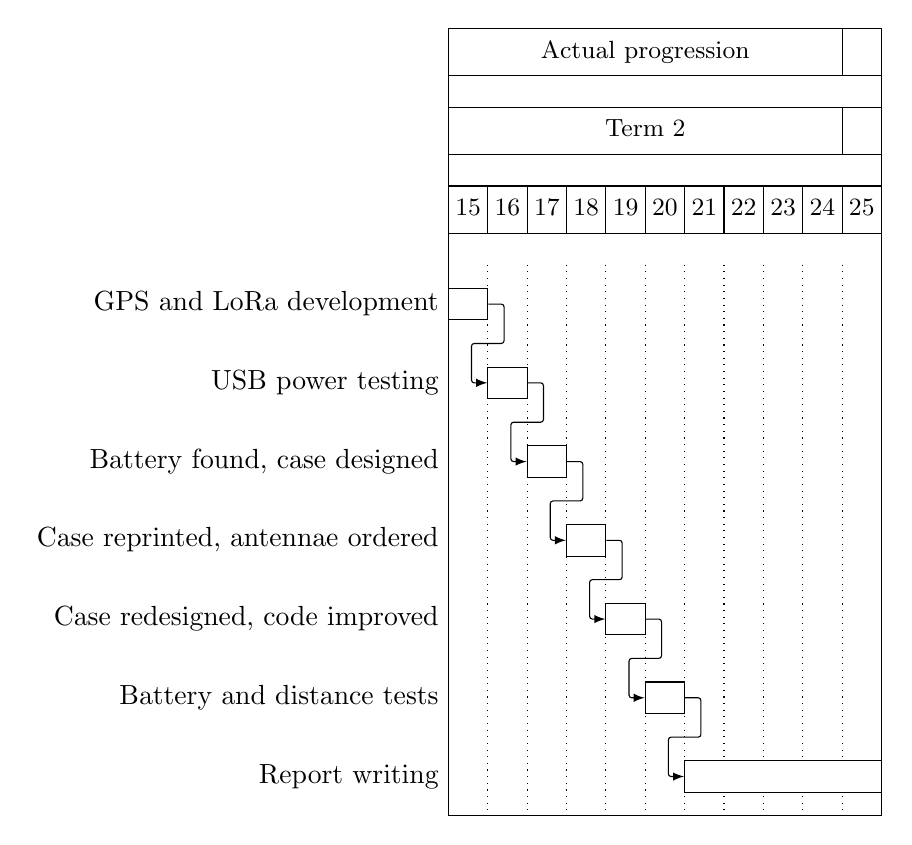
\begin{tikzpicture}[x=.5cm, y=.5cm]
        \begin{ganttchart}[
            % hgrid, 
            vgrid,
            newline shortcut=true,
            % bar inline label node/.append style={right=5mm},
            % milestone inline label node/.append style={align=right}
            group label node/.append style={align=right},
            bar label node/.append style={align=right}
            ]{1}{11}
            \gantttitle{Actual progression}{10} \gantttitle{}{1}\\
            \gantttitle{Term 2}{10} \gantttitle{}{1}\\
            \gantttitlelist{15,...,25}{1} \\
    
            \ganttbar{GPS and LoRa development}{1}{1} \\ 
            \ganttbar{USB power testing}{2}{2} \\
            \ganttbar{Battery found, case designed}{3}{3} \\
            \ganttbar{Case reprinted, antennae ordered}{4}{4} \\
            \ganttbar{Case redesigned, code improved}{5}{5} \\
            \ganttbar{Battery and distance tests}{6}{6} \\
            \ganttbar{Report writing}{7}{11}
        
            \ganttlink{elem0}{elem1}
            \ganttlink{elem1}{elem2}
            \ganttlink{elem2}{elem3}
            \ganttlink{elem3}{elem4}
            \ganttlink{elem4}{elem5}
            \ganttlink{elem5}{elem6}   
        \end{ganttchart}
    \end{tikzpicture}
    }
    \caption{Gantt charts}\label{fig:gantt}
\end{figure}
For context, hardware was only available in mid-December, with development starting in January. 
A more precise breakdown of the course of development can be found in the `Actual progression' Gantt chart 
in \cref{fig:gantt}.
As can be seen, a number of very large developmental steps were taken and refined in a very short span of time. 
The fact that the fundamental aims were soundly met, and subsequently verified is impressive, given the 
very tight timescale upon which it had to happen. 

The progression followed in Term 2 would have been ideal for Term 1, thereby allowing the more 
ambitious and advanced objectives to be met. The plan outlined in the PFS in fact followed this general progression.
This indicates that the initial plan was suitable for this project and likely would have been met, contingent 
on hardware having been available. 

The lesson to be learnt here is that, where any particular aspect (in this case, hardware) is 
so pivotal to the project that progress is impossible without, ensuring mitigations are in place 
\textit{beforehand} is important. For example, alternative hardware could be arranged, or 
development started on existing hardware, with the specific required hardware defined and ordered 
as early as possible. Alternative it could be sourced from elsewhere, without relying on delivery times from 
approved vendors only. 
Finally, if there is no other option than to wait for the hardware to show, the feasibility of the 
project overall needs to be reconsidered. A project that loses half its time simple waiting 
is by no means feasible. 

% \begin{figure}[H]
%     \begin{ganttchart}[
%         hgrid, 
%         vgrid,
%         bar inline label node/.append style={right=5mm},
%         milestone inline label node/.append style={left=5mm}
%         ]{1}{11}
%         \gantttitle{Term start Gantt chart}{10} \gantttitle{}{1}\\
%         \gantttitle{Term 2}{10} \gantttitle{}{1}\\
%         \gantttitlelist{15,...,25}{1} \\
    
%         \ganttgroup{Hardware design}{1}{5} \\
%         \ganttbar{Preliminary battery testing}{1}{1} \\
%         \ganttbar{Hardware order}{1}{1} \ganttbar[inline]{Delivery}{4}{4} \\
%         \ganttbar{Casing and harness design}{2}{3} \\    
%         \ganttbar{Final battery testing}{5}{5} \\
%         \ganttbar{Antenna testing}{5}{5} \\
    
%         \ganttbar{Delay buffer}{6}{8} \\
    
%         \ganttmilestone[inline]{Draft submission}{8} \\ 
%         \ganttbar{Improvements}{9}{10} \\
    
%         \ganttmilestone[inline]{Submission}{10}
    
%         \ganttlink[link type=f-s]{elem1}{elem2}
%         \ganttlink{elem2}{elem3}
%         \ganttlink{elem2}{elem4}
%         \ganttlink[link mid=0.5]{elem3}{elem5}
%         \ganttlink[link mid=0.33]{elem3}{elem6}
%         \ganttlink{elem6}{elem7}
%         \ganttlink{elem7}{elem8}
%         \ganttlink{elem8}{elem9}
%         \ganttlink{elem9}{elem10}    
%     \end{ganttchart}

% \end{figure}

% \begin{figure}[H]
%     \singlespacing
    
%     \begin{ganttchart}[
%         % hgrid, 
%         vgrid,
%         newline shortcut=true,
%         % bar inline label node/.append style={right=5mm},
%         % milestone inline label node/.append style={align=right}
%         group label node/.append style={align=right},
%         bar label node/.append style={align=right}
%         ]{1}{11}
%         \gantttitle{Actual progression}{10} \gantttitle{}{1}\\
%         \gantttitle{Term 2}{10} \gantttitle{}{1}\\
%         \gantttitlelist{15,...,25}{1} \\

%         \ganttbar{GPS and LoRa development}{1}{1} \\ 
%         \ganttbar{USB power testing}{2}{2} \\
%         \ganttbar{Battery found, case designed}{3}{3} \\
%         \ganttbar{Case reprinted, antennae ordered}{4}{4} \\
%         \ganttbar{Case redesigned, code improved}{5}{5} \\
%         \ganttbar{Battery and distance tests}{6}{6} \\
%         \ganttbar{Report writing}{7}{11}
    
%         \ganttlink{elem1}{elem2}
%         \ganttlink{elem2}{elem3}
%         \ganttlink{elem3}{elem4}
%         \ganttlink{elem4}{elem5}
%         \ganttlink{elem5}{elem6}   
%     \end{ganttchart}
% \end{figure}

% \section{Independent work}
% An interesting discovery which is particularly prominent when comparing development plans to the 
% executed procedure, is that at no point were any tasks carried out simultaneously. The Gantt chart 
% in the PFS is particularly rife with tasks occurring simultaneously. While the `actual progression'
% in \cref{fig:gantt} lists multiple tasks occurring in a single block (e.g. ``Battery found, case designed''),
% these tasks were carried out exclusively sequentially. In this instance, the step where the battery was found and 
% appropriate modifications made to allow its use (voltage testing, JST connector changing, etc) was 
% only then followed by developing a case once all the substeps were completed. 

% In short, the project plans created suffered a little from being overly ambitious in how many tasks one person can work on at once,
% and would have benefitted from parcelling tasks out in an explicitly consecutive manner. The 
% planning was overall reasonable and not excessive. The delay buffer provided in particular was helpful for picking 
% up slack, however the large allotment to it suggests a difficulty in accurately timing tasks. 
% The difficulty here may come down to planning for the project in a isolated manner - in other words, as if the project 
% was being carried out in a vacuum and no other tasks or studies were required to be completed at the same time. 
% Again, this comes to the limits of what an individual can complete when not able to solely focus on the project alone. 

% Overall, the plan was still reasonably well thought out, and was followed without major deviation. 

\section{Independent work}
The main areas of non-independent work where advice was sought were in hardware ordering and testing setup. 

In the case of hardware, after producing a shortlist and refining dependent on approved vendors and stock availability, 
the list was then handed off for ordering and not dealt with until the required hardware had arrived. 

Test setup came in two parts. Before purchasing a battery, the expected capacity needed to be determined, 
the advised method of which was to purchase a current tester to measure the characteristics of the transmitter. 
Setting up distance testing also required use of university facilities, and arranging a location in which to 
install the receiver and antenna would have been difficult to do so independently. 

General guidance on reprioritising particular tasks and report writing were greatly appreciated and extremely helpful 
to the overall completion of the project. This was particularly useful in determining tone and direction for written work. 

\section{Feasibility and impact}
Comparing to the project feasibility study performed prior to the commencement of this project, 
many of the identified points hold true. 
The risk register identified health and safety, manufacturing issues, and delays as the 
most significant project risks. In the case of delays, this was referring to failing to 
adhere to the project plan, rather than delivery delays as referred to here. However, 
it ultimately means the project plan could not be followed, so the end result is much the same. 

Health and safety was relevant for testing, due to the nature of electronics. Risk assessments were performed 
before any tests, and overall no issues occurred. Manufacturing issues also occurred, but were 
minimal and easily corrected for.

A major missed expectation of the PFS was live-testing of the tracker with a cat. The subject of ethical 
approval for this to be the case was briefly broached, however the conclusion was that far greater detail 
would be needed in the application, and ultimately it was not carried through in order to save time 
and complete more critical aspects of the project. 

\section{Evaluation}
The three greatest learning experiences of the project are:
\begin{itemize}
    \item Account for hardware delays such that issues with delivery 
            cannot hold the entire project development hostage.
    \item Documentation writing is time-consuming and must be specifically 
            accounted for when creating a development plan. 
    \item Planning cannot be insular, in that other tasks not relevant 
            to the project, but still time-consuming, must be accounted for.
            If they are not, the impression that the plan is poorly thought out
            or the project went of track may result.
\end{itemize}
\medskip
The three greatest positive outcomes are:
\begin{itemize}
    \item The project was completed to a high standard given the time available. While it is regretful 
            that more work could not be done, it is by now means a detractor from the work accomplished.
    \item There was a surprising amount of programming required for this project. This was expected for 
            the tracker, however less expected was the plotting programming requirements. In any case, the 
            end result were appropriate and professional, while clear graphs and charts across the board. 
    \item The greatest outcome is that the tracker does in fact work, and rather well at that. While the 
            precise limits have not been characterised, it is suitable for tracking within most owned cats' 
            home ranges. To make a minimum viable product, all that is needed is a waterproof casing, 
            which is fairly simple to design. 
\end{itemize}

\paragraph{Completed work}
A functioning tracker, with a small amount of refinement required to get serviceable. 
The system requirements were defined and used to inform hardware purchasing decisions. Once the hardware 
arrived, it was soldered and then programmed. Programming overall progressed smoothly, with the only 
issue being the occasional crash on the receiver end which was then handled safely. 
A case was designed and then updated using findings from the first design. 
Tests were designed for the tracker, and it was found to perform fairly well in these tests. 
Overall, a relatively successful outcome.

\paragraph{Future work}
There are some points that would be taken on in future work. More testing to completely characterise the tracker,
before working to minimise the size of the transmitter. The receiver would not be too complex to modify such that 
it can store data in a database and serve a web frontend for the user to view live location overlaid on a map. 
One of the key takeaways from this project is effectively managing when things do not go to plan externally. 
For example, producing a backup plan of work where a critical factor (like hardware) is unavailable.

\end{document}